\documentclass[tikz,border=8pt]{standalone}
\usepackage{amsmath,amssymb}
\usetikzlibrary{arrows.meta,automata,positioning,quotes}
\begin{document}
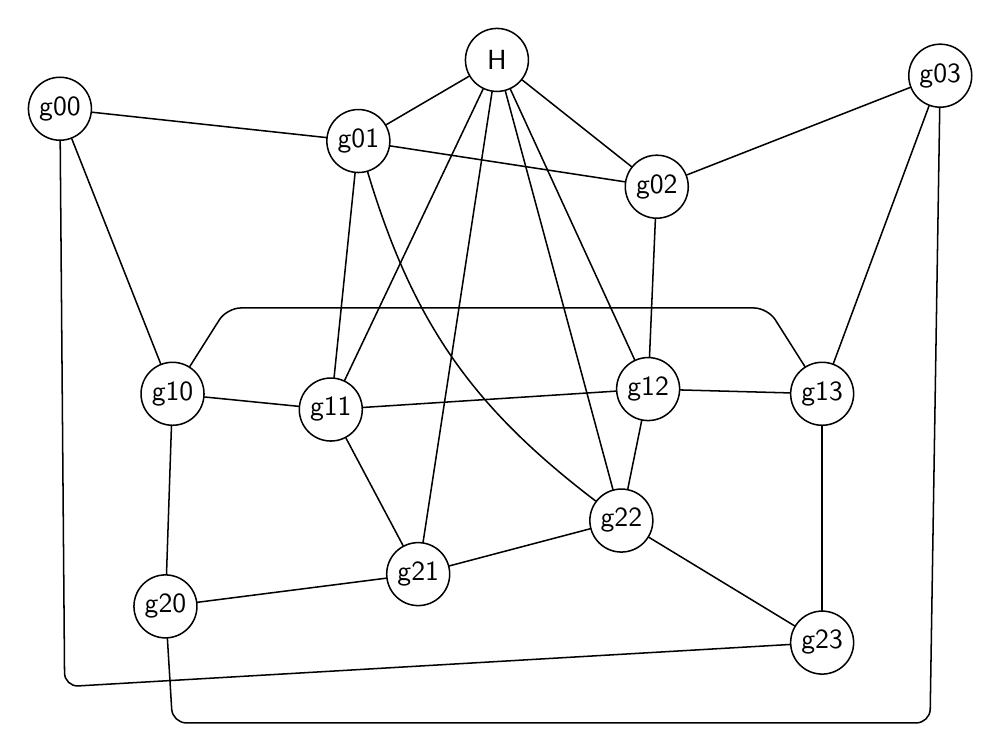
\begin{tikzpicture}[x=1cm,y=1cm]
\tikzset{
  graphnode/.style={circle,draw=black,line width=0.55pt,minimum size=8mm,inner sep=1pt,font=\sffamily},
  graphedge/.style={draw=black,line width=0.55pt,line cap=round,line join=round},
  directed/.style={graphedge,-{Stealth[length=2.4mm,width=2.0mm]}},
  undirected/.style={graphedge}
}
\node[graphnode] (n_g00) at (-1.96,3.49) {g00};
\node[graphnode] (n_g01) at (1.83,3.08) {g01};
\node[graphnode] (n_g02) at (5.62,2.50) {g02};
\node[graphnode] (n_g03) at (9.22,3.91) {g03};
\node[graphnode] (n_g10) at (-0.53,-0.13) {g10};
\node[graphnode] (n_g11) at (1.48,-0.33) {g11};
\node[graphnode] (n_g12) at (5.51,-0.07) {g12};
\node[graphnode] (n_g13) at (7.72,-0.13) {g13};
\node[graphnode] (n_g20) at (-0.62,-2.83) {g20};
\node[graphnode] (n_g21) at (2.59,-2.42) {g21};
\node[graphnode] (n_g22) at (5.17,-1.74) {g22};
\node[graphnode] (n_g23) at (7.72,-3.29) {g23};
\node[graphnode] (n_H) at (3.59,4.11) {H};
\draw[undirected] (n_g00) -- (n_g01);
\draw[undirected] (n_g01) -- (n_g02);
\draw[undirected] (n_g02) -- (n_g03);
\draw[undirected] (n_g10) -- (n_g11);
\draw[undirected] (n_g11) -- (n_g12);
\draw[undirected] (n_g12) -- (n_g13);
\draw[undirected] (n_g20) -- (n_g21);
\draw[undirected] (n_g21) -- (n_g22);
\draw[undirected] (n_g22) -- (n_g23);
\draw[undirected] (n_g00) -- (n_g10);
\draw[undirected] (n_g10) -- (n_g20);
\draw[undirected] (n_g01) -- (n_g11);
\draw[undirected] (n_g11) -- (n_g21);
\draw[undirected] (n_g02) -- (n_g12);
\draw[undirected] (n_g12) -- (n_g22);
\draw[undirected] (n_g03) -- (n_g13);
\draw[undirected] (n_g13) -- (n_g23);
\draw[undirected] (n_H) -- (n_g01);
\draw[undirected] (n_H) -- (n_g02);
\draw[undirected] (n_H) -- (n_g11);
\draw[undirected] (n_H) -- (n_g12);
\draw[undirected] (n_H) -- (n_g21);
\draw[undirected] (n_H) -- (n_g22);
\draw[undirected,rounded corners=5pt] (n_g00) -- (-1.90,-3.85) -- (n_g23);
\draw[undirected,rounded corners=5pt] (n_g03) -- (9.09,-4.31) -- (-0.53,-4.31) -- (n_g20);
\draw[undirected,rounded corners=5pt] (n_g10) -- (0.16,0.96) -- (7.03,0.96) -- (n_g13);
\draw[undirected] (n_g01) to[bend right=18] (n_g22);
\end{tikzpicture}
\end{document}
